\documentclass{whiteboard}
\begin{document}
\begin{frame}[plain,t]
 \bbcover{Grafos}{Algoritmo de Dijkstra}{Prof. Edson Alves}{Faculdade UnB Gama}
\end{frame}

\begin{frame}[plain,t]
\begin{tikzpicture}
\node[draw,opacity=0] at (0, 0) {x};
\node[draw,opacity=0] at (14, 8) {x};
 \node[anchor=west] at (0, 7) { \Large \bbbold{Proponente} };
\end{tikzpicture}
\end{frame}

\begin{frame}[plain,t]
\begin{tikzpicture}
\node[draw,opacity=0] at (0, 0) {x};
\node[draw,opacity=0] at (14, 8) {x};
 \node[anchor=west] at (0, 7) { \Large \bbbold{Proponente} };
 \node at (7, 4.5) { \includegraphics[scale=0.45]{figs/dijkstra.jpg} };
 \node at (7, 1.5) { \bbbold{Edsger Wybe Dijkstra} };
 \node at (7, 1.0) { \bbtext{(1956)} };
\end{tikzpicture}
\end{frame}

\begin{frame}[plain,t]
\begin{tikzpicture}
\node[draw,opacity=0] at (0, 0) {x};
\node[draw,opacity=0] at (14, 8) {x};
 \node[anchor=west] at (0, 6) { \Large \bbbold{Características do algoritmo de Dijkstra } };
\end{tikzpicture}
\end{frame}

\begin{frame}[plain,t]
\begin{tikzpicture}
\node[draw,opacity=0] at (0, 0) {x};
\node[draw,opacity=0] at (14, 8) {x};
 \node[anchor=west] at (0, 6) { \Large \bbbold{Características do algoritmo de Dijkstra } };
 \node[anchor=west] at (0.5, 5) { $\star$ \bbtext{Computa o caminho mínimo de todos os vértices de $G(V, E)$ a um dado nó $s$} };
\end{tikzpicture}
\end{frame}

\begin{frame}[plain,t]
\begin{tikzpicture}
\node[draw,opacity=0] at (0, 0) {x};
\node[draw,opacity=0] at (14, 8) {x};
 \node[anchor=west] at (0, 6) { \Large \bbbold{Características do algoritmo de Dijkstra } };
 \node[anchor=west] at (0.5, 5) { $\star$ \bbtext{Computa o caminho mínimo de todos os vértices de $G(V, E)$ a um dado nó $s$} };
 \node[anchor=west] at (0.5, 4) { $\star$ \bbtext{Processa corretamente apenas grafos com arestas não-negativas} };
\end{tikzpicture}
\end{frame}

\begin{frame}[plain,t]
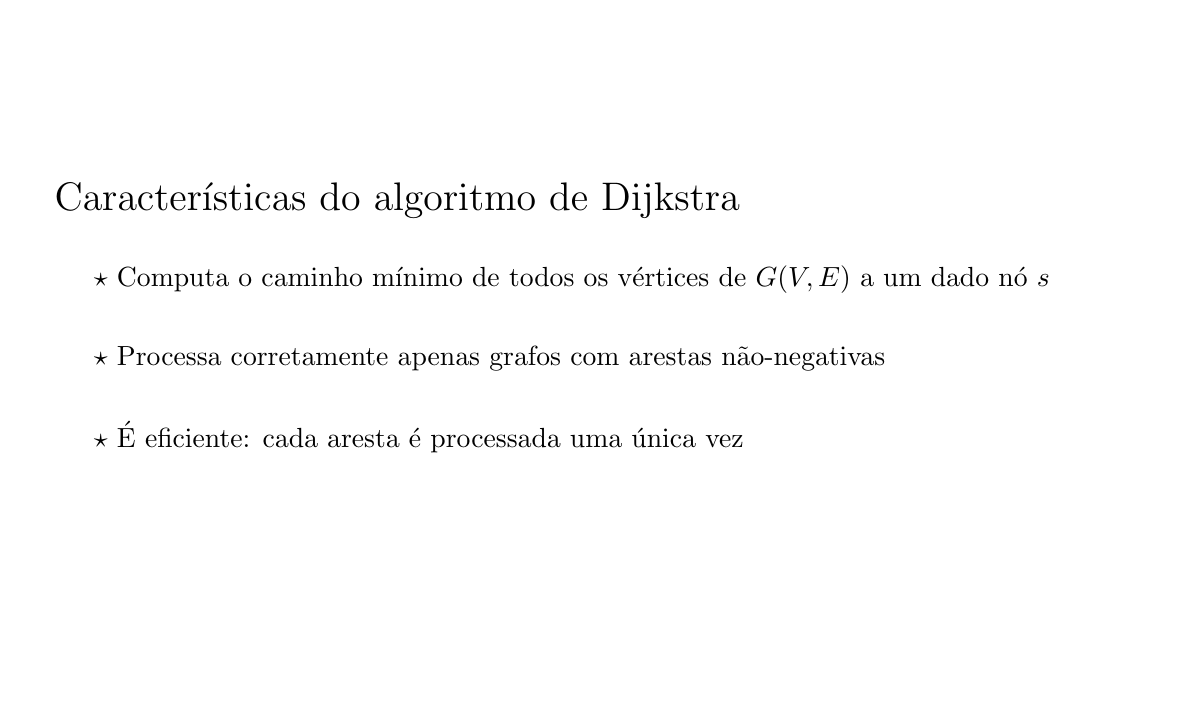
\begin{tikzpicture}
\node[draw,opacity=0] at (0, 0) {x};
\node[draw,opacity=0] at (14, 8) {x};
 \node[anchor=west] at (0, 6) { \Large \bbbold{Características do algoritmo de Dijkstra } };
 \node[anchor=west] at (0.5, 5) { $\star$ \bbtext{Computa o caminho mínimo de todos os vértices de $G(V, E)$ a um dado nó $s$} };
 \node[anchor=west] at (0.5, 4) { $\star$ \bbtext{Processa corretamente apenas grafos com arestas não-negativas} };
 \node[anchor=west] at (0.5, 3) { $\star$ \bbtext{É eficiente: cada aresta é processada uma única vez} };
\end{tikzpicture}
\end{frame}

\begin{frame}[plain,t]
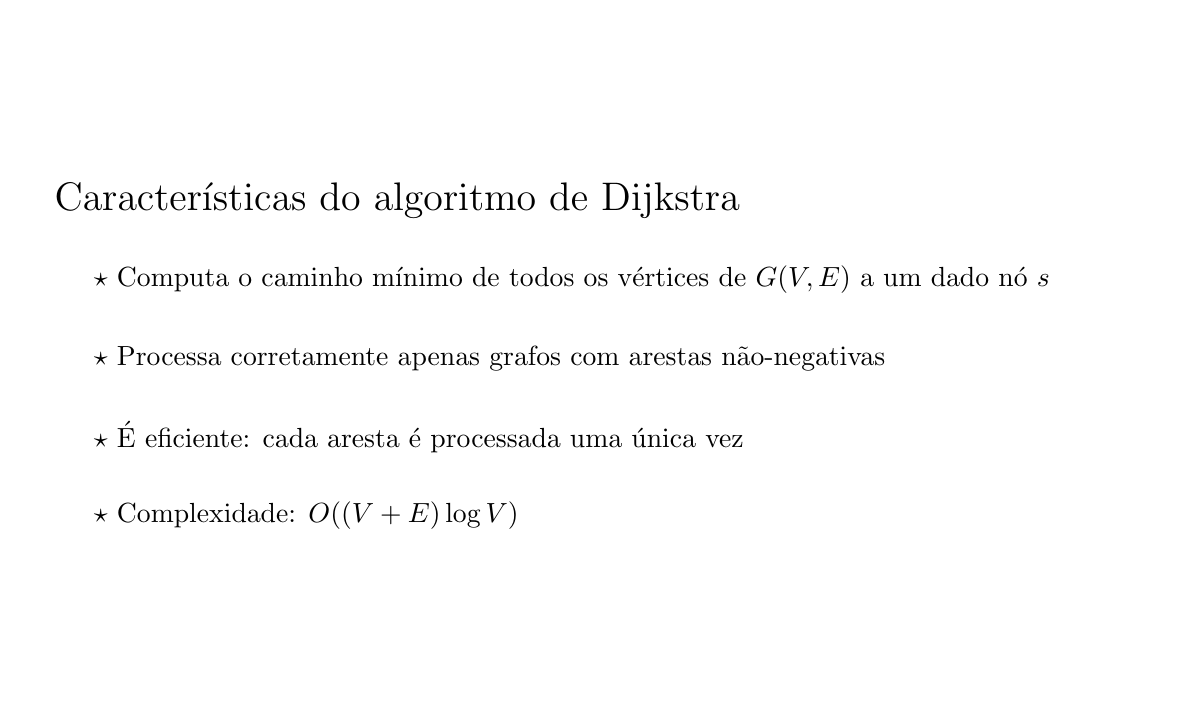
\begin{tikzpicture}
\node[draw,opacity=0] at (0, 0) {x};
\node[draw,opacity=0] at (14, 8) {x};
 \node[anchor=west] at (0, 6) { \Large \bbbold{Características do algoritmo de Dijkstra } };
 \node[anchor=west] at (0.5, 5) { $\star$ \bbtext{Computa o caminho mínimo de todos os vértices de $G(V, E)$ a um dado nó $s$} };
 \node[anchor=west] at (0.5, 4) { $\star$ \bbtext{Processa corretamente apenas grafos com arestas não-negativas} };
 \node[anchor=west] at (0.5, 3) { $\star$ \bbtext{É eficiente: cada aresta é processada uma única vez} };
 \node[anchor=west] at (0.5, 2) { $\star$ \bbtext{\bbbold{Complexidade}: $O((V + E)\log V)$ } };
\end{tikzpicture}
\end{frame}

\begin{frame}[plain,t]
\begin{tikzpicture}
\node[draw,opacity=0] at (0, 0) {x};
\node[draw,opacity=0] at (14, 8) {x};
 \node[anchor=west] at (0, 7) { \Large \bbbold{Pseudocódigo } };
\end{tikzpicture}
\end{frame}

\begin{frame}[plain,t]
\begin{tikzpicture}
\node[draw,opacity=0] at (0, 0) {x};
\node[draw,opacity=0] at (14, 8) {x};
 \node[anchor=west] at (0, 7) { \Large \bbbold{Pseudocódigo } };
 \node[anchor=west] at (0, 6) { \bbemph{Entrada:} \bbtext{um grafo $G(V, E)$ e um vértice $s\in V$} };
 \node[anchor=west] at (0, 5.5) { \bbemph{Saída:} \bbtext{um vetor $d$ tal que $d[u]$ é a distância mínima em $G$ entre $s$ e $u$ } };
\end{tikzpicture}
\end{frame}

\begin{frame}[plain,t]
\begin{tikzpicture}
\node[draw,opacity=0] at (0, 0) {x};
\node[draw,opacity=0] at (14, 8) {x};
 \node[anchor=west] at (0, 7) { \Large \bbbold{Pseudocódigo } };
 \node[anchor=west] at (0, 6) { \bbemph{Entrada:} \bbtext{um grafo $G(V, E)$ e um vértice $s\in V$} };
 \node[anchor=west] at (0, 5.5) { \bbemph{Saída:} \bbtext{um vetor $d$ tal que $d[u]$ é a distância mínima em $G$ entre $s$ e $u$ } };
 \node[anchor=west] at (1.0, 4.5) { $1.$ \bbtext{Faça $d[s] = 0$, $d[u] = \infty$ se $u\neq s$ e seja $U = V$}};
\end{tikzpicture}
\end{frame}

\begin{frame}[plain,t]
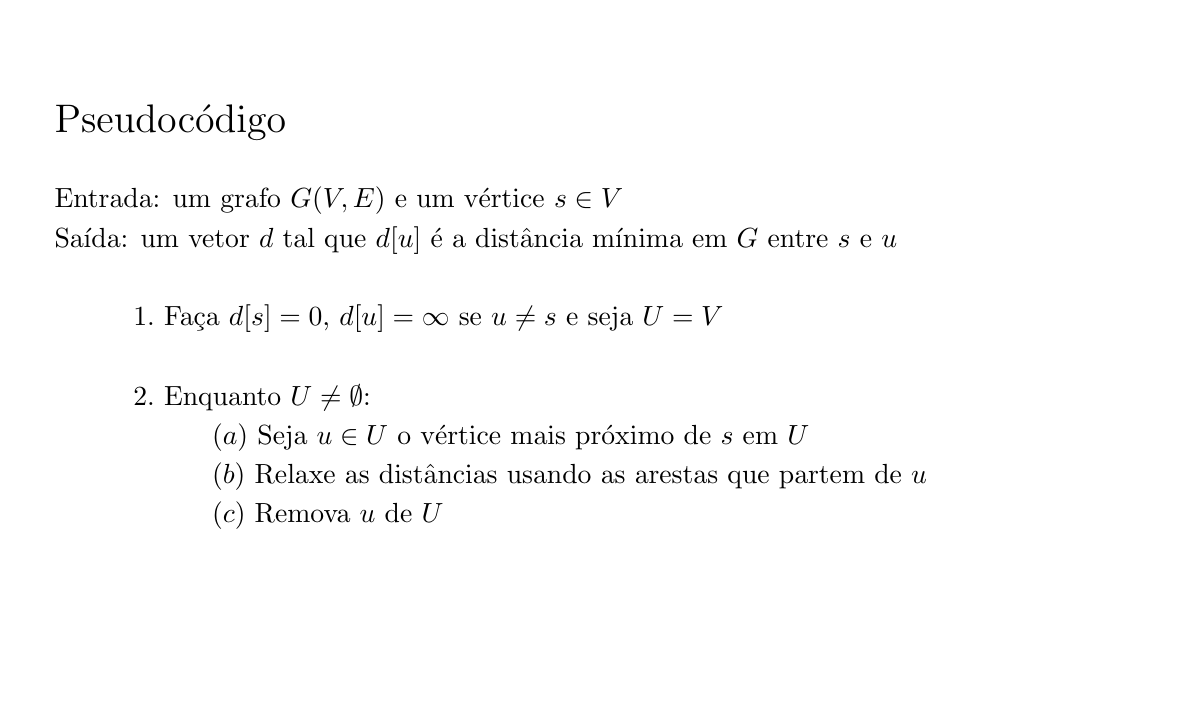
\begin{tikzpicture}
\node[draw,opacity=0] at (0, 0) {x};
\node[draw,opacity=0] at (14, 8) {x};
 \node[anchor=west] at (0, 7) { \Large \bbbold{Pseudocódigo } };
 \node[anchor=west] at (0, 6) { \bbemph{Entrada:} \bbtext{um grafo $G(V, E)$ e um vértice $s\in V$} };
 \node[anchor=west] at (0, 5.5) { \bbemph{Saída:} \bbtext{um vetor $d$ tal que $d[u]$ é a distância mínima em $G$ entre $s$ e $u$ } };
 \node[anchor=west] at (1.0, 4.5) { $1.$ \bbtext{Faça $d[s] = 0$, $d[u] = \infty$ se $u\neq s$ e seja $U = V$}};
 \node[anchor=west] at (1.0, 3.5) { $2.$ \bbtext{Enquanto $U\neq \emptyset$:} };
 \node[anchor=west] at (2.0, 3.0) { $(a)$ \bbtext{Seja $u\in U$ o vértice mais próximo de $s$ em $U$} };
 \node[anchor=west] at (2.0, 2.5) { $(b)$ \bbtext{Relaxe as distâncias usando as arestas que partem de $u$ } };
 \node[anchor=west] at (2.0, 2.0) { $(c)$ \bbtext{Remova $u$ de $U$ } };
\end{tikzpicture}
\end{frame}

\begin{frame}[plain,t]
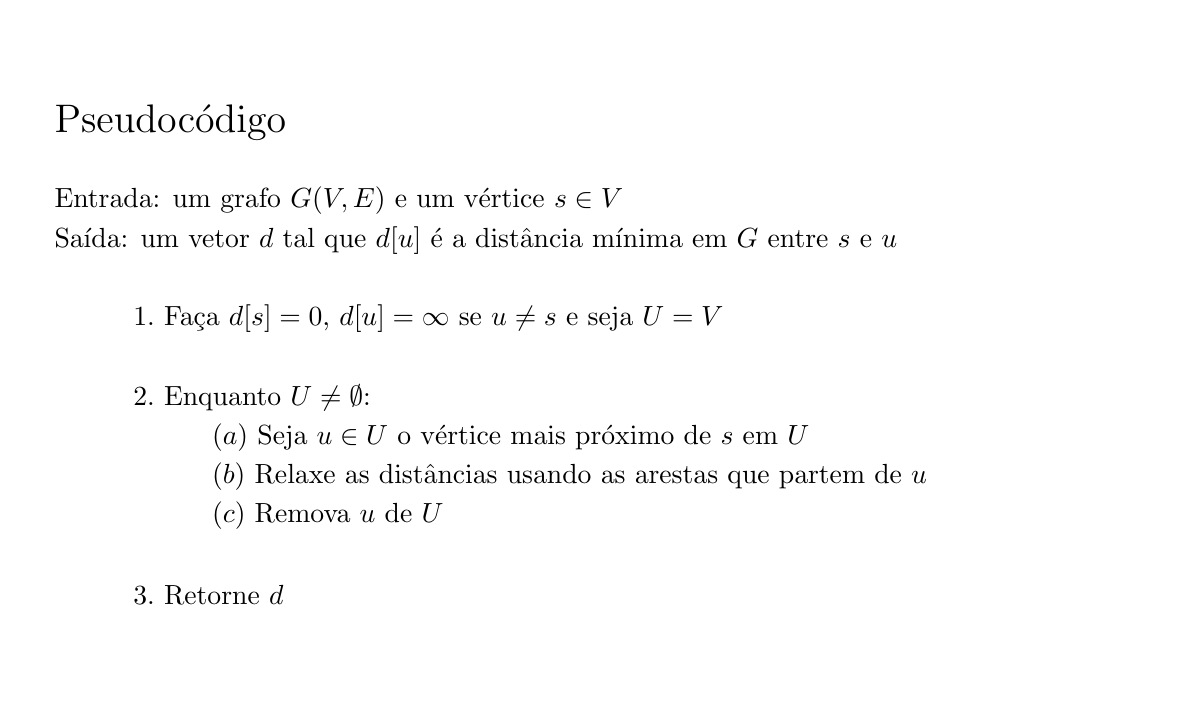
\begin{tikzpicture}
\node[draw,opacity=0] at (0, 0) {x};
\node[draw,opacity=0] at (14, 8) {x};
 \node[anchor=west] at (0, 7) { \Large \bbbold{Pseudocódigo } };
 \node[anchor=west] at (0, 6) { \bbemph{Entrada:} \bbtext{um grafo $G(V, E)$ e um vértice $s\in V$} };
 \node[anchor=west] at (0, 5.5) { \bbemph{Saída:} \bbtext{um vetor $d$ tal que $d[u]$ é a distância mínima em $G$ entre $s$ e $u$ } };
 \node[anchor=west] at (1.0, 4.5) { $1.$ \bbtext{Faça $d[s] = 0$, $d[u] = \infty$ se $u\neq s$ e seja $U = V$}};
 \node[anchor=west] at (1.0, 3.5) { $2.$ \bbtext{Enquanto $U\neq \emptyset$:} };
 \node[anchor=west] at (2.0, 3.0) { $(a)$ \bbtext{Seja $u\in U$ o vértice mais próximo de $s$ em $U$} };
 \node[anchor=west] at (2.0, 2.5) { $(b)$ \bbtext{Relaxe as distâncias usando as arestas que partem de $u$ } };
 \node[anchor=west] at (2.0, 2.0) { $(c)$ \bbtext{Remova $u$ de $U$ } };
 \node[anchor=west] at (1.0, 1.0) { $3.$ \bbtext{Retorne $d$ } };
\end{tikzpicture}
\end{frame}

\begin{frame}[plain,t]
\begin{tikzpicture}
\node[draw,opacity=0] at (0, 0) {x};
\node[draw,opacity=0] at (14, 8) {x};
 \node[anchor=west] at (0, 7) { \Large \bbbold{Relaxamento} };
\end{tikzpicture}
\end{frame}

\begin{frame}[plain,t]
\begin{tikzpicture}
\node[draw,opacity=0] at (0, 0) {x};
\node[draw,opacity=0] at (14, 8) {x};
 \node[anchor=west] at (0, 7) { \Large \bbbold{Relaxamento} };
 \node[circle, draw, very thick] (s) at (2, 4) { $s$ };
 \node[circle, draw, very thick] (a) at (4, 6) { $a$ };
 \node[circle, draw, very thick] (b) at (6, 5) { $b$ };
 \node[circle, draw, very thick] (c) at (8, 7) { $c$ };
 \node[circle, draw, very thick] (d) at (4, 3) { $c$ };
 \node[circle, draw, very thick] (u) at (10, 6) { $u$ };
 \node[circle, draw, very thick] (v) at (12, 3) { $v$ };
 \draw[-latex,very thick,color=BBCyan] (s) to node[above left] { $r_1$ } (a);
 \draw[-latex,very thick,color=BBCyan] (a) to node[above right] { $r_2$ } (b);
 \draw[-latex,very thick,color=BBCyan] (b) to node[above left] { $r_3$ } (c);
 \draw[-latex,very thick,color=BBCyan] (c) to node[above right] { $r_4$ } (u);
 \draw[-latex,very thick,color=BBViolet] (s) to node[below] { $s_1$ } (b);
 \draw[-latex,very thick,color=BBViolet] (b) to node[below right] { $s_2$ } (d);
 \draw[-latex,very thick,color=BBViolet] (d) to node[below] { $s_3$ } (v);
\end{tikzpicture}
\end{frame}

\begin{frame}[plain,t]
\begin{tikzpicture}
\node[draw,opacity=0] at (0, 0) {x};
\node[draw,opacity=0] at (14, 8) {x};
 \node[anchor=west] at (0, 7) { \Large \bbbold{Relaxamento} };
 \node[circle, draw, very thick] (s) at (2, 4) { $s$ };
 \node[circle, draw, very thick] (a) at (4, 6) { $a$ };
 \node[circle, draw, very thick] (b) at (6, 5) { $b$ };
 \node[circle, draw, very thick] (c) at (8, 7) { $c$ };
 \node[circle, draw, very thick] (d) at (4, 3) { $c$ };
 \node[circle, draw, very thick] (u) at (10, 6) { $u$ };
 \node[circle, draw, very thick] (v) at (12, 3) { $v$ };
 \draw[-latex,very thick,color=BBCyan] (s) to node[above left] { $r_1$ } (a);
 \draw[-latex,very thick,color=BBCyan] (a) to node[above right] { $r_2$ } (b);
 \draw[-latex,very thick,color=BBCyan] (b) to node[above left] { $r_3$ } (c);
 \draw[-latex,very thick,color=BBCyan] (c) to node[above right] { $r_4$ } (u);
 \draw[-latex,very thick,color=BBViolet] (s) to node[below] { $s_1$ } (b);
 \draw[-latex,very thick,color=BBViolet] (b) to node[below right] { $s_2$ } (d);
 \draw[-latex,very thick,color=BBViolet] (d) to node[below] { $s_3$ } (v);
 \node[anchor=west] at (2, 1.5) { $\displaystyle{\dist(s, u) = \sum_{i = 1}^4 r_i}$ };
 \node[anchor=west] at (7, 1.5) { $\displaystyle{\dist(s, v) = \sum_{j = 1}^3 s_i}$ };
\end{tikzpicture}
\end{frame}

\begin{frame}[plain,t]
\begin{tikzpicture}
\node[draw,opacity=0] at (0, 0) {x};
\node[draw,opacity=0] at (14, 8) {x};
 \node[anchor=west] at (0, 7) { \Large \bbbold{Relaxamento} };
 \node[circle, draw, very thick] (s) at (2, 4) { $s$ };
 \node[circle, draw, very thick] (a) at (4, 6) { $a$ };
 \node[circle, draw, very thick] (b) at (6, 5) { $b$ };
 \node[circle, draw, very thick] (c) at (8, 7) { $c$ };
 \node[circle, draw, very thick] (d) at (4, 3) { $c$ };
 \node[circle, draw, very thick] (u) at (10, 6) { $u$ };
 \node[circle, draw, very thick] (v) at (12, 3) { $v$ };
 \draw[-latex,very thick,color=BBCyan] (s) to node[above left] { $r_1$ } (a);
 \draw[-latex,very thick,color=BBCyan] (a) to node[above right] { $r_2$ } (b);
 \draw[-latex,very thick,color=BBCyan] (b) to node[above left] { $r_3$ } (c);
 \draw[-latex,very thick,color=BBCyan] (c) to node[above right] { $r_4$ } (u);
 \draw[-latex,very thick,color=BBViolet] (s) to node[below] { $s_1$ } (b);
 \draw[-latex,very thick,color=BBViolet] (b) to node[below right] { $s_2$ } (d);
 \draw[-latex,very thick,color=BBViolet] (d) to node[below] { $s_3$ } (v);
 \draw[-latex,very thick,color=BBRed] (u) to node[above right] { $w$ } (v);
\end{tikzpicture}
\end{frame}

\begin{frame}[plain,t]
\begin{tikzpicture}
\node[draw,opacity=0] at (0, 0) {x};
\node[draw,opacity=0] at (14, 8) {x};
 \node[anchor=west] at (0, 7) { \Large \bbbold{Relaxamento} };
 \node[circle, draw, very thick] (s) at (2, 4) { $s$ };
 \node[circle, draw, very thick] (a) at (4, 6) { $a$ };
 \node[circle, draw, very thick] (b) at (6, 5) { $b$ };
 \node[circle, draw, very thick] (c) at (8, 7) { $c$ };
 \node[circle, draw, very thick] (d) at (4, 3) { $c$ };
 \node[circle, draw, very thick] (u) at (10, 6) { $u$ };
 \node[circle, draw, very thick] (v) at (12, 3) { $v$ };
 \draw[-latex,very thick,color=BBCyan] (s) to node[above left] { $r_1$ } (a);
 \draw[-latex,very thick,color=BBCyan] (a) to node[above right] { $r_2$ } (b);
 \draw[-latex,very thick,color=BBCyan] (b) to node[above left] { $r_3$ } (c);
 \draw[-latex,very thick,color=BBCyan] (c) to node[above right] { $r_4$ } (u);
 \draw[-latex,very thick,color=BBViolet] (s) to node[below] { $s_1$ } (b);
 \draw[-latex,very thick,color=BBViolet] (b) to node[below right] { $s_2$ } (d);
 \draw[-latex,very thick,color=BBViolet] (d) to node[below] { $s_3$ } (v);
 \draw[-latex,very thick,color=BBRed] (u) to node[above right] { $w$ } (v);
 \node[anchor=west] at (2, 1.5) { \bbtext{Se $\dist(s, u) + w < \dist(s, v)$, faça $\dist(s, v) = \dist(s, u) + w$} };
\end{tikzpicture}
\end{frame}

\begin{frame}[plain,t]
\begin{tikzpicture}
\node[draw,opacity=0] at (0, 0) {x};
\node[draw,opacity=0] at (14, 8) {x};
 \node[circle, draw, very thick] (A) at (5, 7.5) { \bbtext{A} };
 \node[circle, draw, very thick] (B) at (2, 5.5) { \bbtext{B} };
 \node[circle, draw, very thick] (C) at (5, 3.5) { \bbtext{C} };
 \node[circle, draw, very thick] (D) at (8, 7.5) { \bbtext{D} };
 \node[circle, draw, very thick] (E) at (11, 5.5) { \bbtext{E} };
 \node[circle, draw, very thick] (F) at (8, 3.5) { \bbtext{F} };
 \draw[thick] (A) to node[above] { \bbinfo{9} } (B);
 \draw[thick] (A) to node[right] { \bbinfo{7} } (C);
 \draw[thick] (A) to node[above] { \bbinfo{4} } (D);
 \draw[thick] (A) to node[below] { \bbinfo{2} } (E);
 \draw[thick] (B) to node[below] { \bbinfo{1} } (C);
 \draw[thick] (B) to node[below,pos=0.8] { \bbinfo{3} } (F);
 \draw[thick] (C) to node[right] { \bbinfo{2} } (D);
 \draw[thick] (D) to node[above] { \bbinfo{1} } (E);
 \draw[thick] (E) to node[below] { \bbinfo{11} } (F);
\end{tikzpicture}
\end{frame}

\begin{frame}[plain,t]
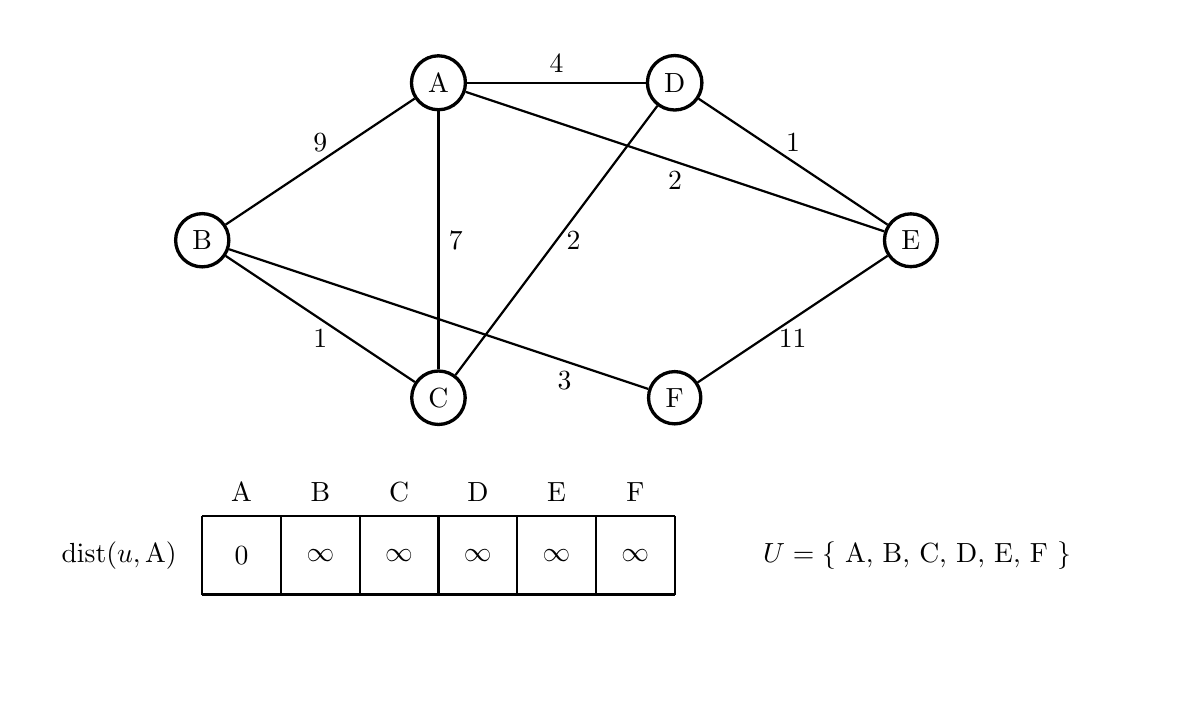
\begin{tikzpicture}
\node[draw,opacity=0] at (0, 0) {x};
\node[draw,opacity=0] at (14, 8) {x};
 \node[circle, draw, very thick] (A) at (5, 7.5) { \bbtext{A} };
 \node[circle, draw, very thick] (B) at (2, 5.5) { \bbtext{B} };
 \node[circle, draw, very thick] (C) at (5, 3.5) { \bbtext{C} };
 \node[circle, draw, very thick] (D) at (8, 7.5) { \bbtext{D} };
 \node[circle, draw, very thick] (E) at (11, 5.5) { \bbtext{E} };
 \node[circle, draw, very thick] (F) at (8, 3.5) { \bbtext{F} };
 \draw[thick] (A) to node[above] { \bbinfo{9} } (B);
 \draw[thick] (A) to node[right] { \bbinfo{7} } (C);
 \draw[thick] (A) to node[above] { \bbinfo{4} } (D);
 \draw[thick] (A) to node[below] { \bbinfo{2} } (E);
 \draw[thick] (B) to node[below] { \bbinfo{1} } (C);
 \draw[thick] (B) to node[below,pos=0.8] { \bbinfo{3} } (F);
 \draw[thick] (C) to node[right] { \bbinfo{2} } (D);
 \draw[thick] (D) to node[above] { \bbinfo{1} } (E);
 \draw[thick] (E) to node[below] { \bbinfo{11} } (F);
 \draw[thick] (2, 1) grid (8, 2);
 \node[anchor=east] at (1.8, 1.5) { $\mathrm{dist}(u, \mbox{\bbtext{A}})$ };
 \node at (2.5, 2.3) { \bbtext{A} };
 \node at (3.5, 2.3) { \bbtext{B} };
 \node at (4.5, 2.3) { \bbtext{C} };
 \node at (5.5, 2.3) { \bbtext{D} };
 \node at (6.5, 2.3) { \bbtext{E} };
 \node at (7.5, 2.3) { \bbtext{F} };
 \node at (2.5, 1.5) { $0$ };
 \node at (3.5, 1.5) { $\infty$ };
 \node at (4.5, 1.5) { $\infty$ };
 \node at (5.5, 1.5) { $\infty$ };
 \node at (6.5, 1.5) { $\infty$ };
 \node at (7.5, 1.5) { $\infty$ };
 \node[anchor=west] at (9, 1.5) { \bbtext{$U = \{$ A, B, C, D, E, F $\}$ } };
\end{tikzpicture}
\end{frame}

\begin{frame}[plain,t]
\begin{tikzpicture}
\node[draw,opacity=0] at (0, 0) {x};
\node[draw,opacity=0] at (14, 8) {x};
 \node[circle, draw, very thick] (B) at (2, 5.5) { \bbtext{B} };
 \node[circle, draw, very thick] (C) at (5, 3.5) { \bbtext{C} };
 \node[circle, draw, very thick] (D) at (8, 7.5) { \bbtext{D} };
 \node[circle, draw, very thick] (E) at (11, 5.5) { \bbtext{E} };
 \node[circle, draw, very thick] (F) at (8, 3.5) { \bbtext{F} };
 \draw[thick] (A) to node[above] { \bbinfo{9} } (B);
 \draw[thick] (A) to node[right] { \bbinfo{7} } (C);
 \draw[thick] (A) to node[above] { \bbinfo{4} } (D);
 \draw[thick] (A) to node[below] { \bbinfo{2} } (E);
 \draw[thick] (B) to node[below] { \bbinfo{1} } (C);
 \draw[thick] (B) to node[below,pos=0.8] { \bbinfo{3} } (F);
 \draw[thick] (C) to node[right] { \bbinfo{2} } (D);
 \draw[thick] (D) to node[above] { \bbinfo{1} } (E);
 \draw[thick] (E) to node[below] { \bbinfo{11} } (F);
 \draw[thick] (2, 1) grid (8, 2);
 \node[anchor=east] at (1.8, 1.5) { $\mathrm{dist}(u, \mbox{\bbtext{A}})$ };
 \node at (2.5, 2.3) { \bbtext{A} };
 \node at (3.5, 2.3) { \bbtext{B} };
 \node at (4.5, 2.3) { \bbtext{C} };
 \node at (5.5, 2.3) { \bbtext{D} };
 \node at (6.5, 2.3) { \bbtext{E} };
 \node at (7.5, 2.3) { \bbtext{F} };
 \node at (2.5, 1.5) { $0$ };
 \node at (3.5, 1.5) { $\infty$ };
 \node at (4.5, 1.5) { $\infty$ };
 \node at (5.5, 1.5) { $\infty$ };
 \node at (6.5, 1.5) { $\infty$ };
 \node at (7.5, 1.5) { $\infty$ };
 \node[circle, draw, very thick,fill=BBGreen] (A) at (5, 7.5) { \bbtext{A} };
 \node[anchor=west] at (9, 1.5) { \bbtext{$U = \{$ B, C, D, E, F $\}$ } };
\end{tikzpicture}
\end{frame}

\begin{frame}[plain,t]
\begin{tikzpicture}
\node[draw,opacity=0] at (0, 0) {x};
\node[draw,opacity=0] at (14, 8) {x};
 \node[circle, draw, very thick] (B) at (2, 5.5) { \bbtext{B} };
 \node[circle, draw, very thick] (C) at (5, 3.5) { \bbtext{C} };
 \node[circle, draw, very thick] (D) at (8, 7.5) { \bbtext{D} };
 \node[circle, draw, very thick] (E) at (11, 5.5) { \bbtext{E} };
 \node[circle, draw, very thick] (F) at (8, 3.5) { \bbtext{F} };
 \draw[thick] (A) to node[right] { \bbinfo{7} } (C);
 \draw[thick] (A) to node[above] { \bbinfo{4} } (D);
 \draw[thick] (A) to node[below] { \bbinfo{2} } (E);
 \draw[thick] (B) to node[below] { \bbinfo{1} } (C);
 \draw[thick] (B) to node[below,pos=0.8] { \bbinfo{3} } (F);
 \draw[thick] (C) to node[right] { \bbinfo{2} } (D);
 \draw[thick] (D) to node[above] { \bbinfo{1} } (E);
 \draw[thick] (E) to node[below] { \bbinfo{11} } (F);
 \draw[thick] (2, 1) grid (8, 2);
 \node[anchor=east] at (1.8, 1.5) { $\mathrm{dist}(u, \mbox{\bbtext{A}})$ };
 \node at (2.5, 2.3) { \bbtext{A} };
 \node at (3.5, 2.3) { \bbtext{B} };
 \node at (4.5, 2.3) { \bbtext{C} };
 \node at (5.5, 2.3) { \bbtext{D} };
 \node at (6.5, 2.3) { \bbtext{E} };
 \node at (7.5, 2.3) { \bbtext{F} };
 \node at (2.5, 1.5) { $0$ };
 \node at (4.5, 1.5) { $\infty$ };
 \node at (5.5, 1.5) { $\infty$ };
 \node at (6.5, 1.5) { $\infty$ };
 \node at (7.5, 1.5) { $\infty$ };
 \node[circle, draw, very thick,fill=BBGreen] (A) at (5, 7.5) { \bbtext{A} };
 \node[anchor=west] at (9, 1.5) { \bbtext{$U = \{$ B, C, D, E, F $\}$ } };
 \draw[-latex,color=BBCyan,very thick] (A) to node[above] { \bbinfo{9} } (B);
 \node at (3.5, 1.5) { $\mathbf{9}$ };
\end{tikzpicture}
\end{frame}

\begin{frame}[plain,t]
\begin{tikzpicture}
\node[draw,opacity=0] at (0, 0) {x};
\node[draw,opacity=0] at (14, 8) {x};
 \node[circle, draw, very thick] (B) at (2, 5.5) { \bbtext{B} };
 \node[circle, draw, very thick] (C) at (5, 3.5) { \bbtext{C} };
 \node[circle, draw, very thick] (D) at (8, 7.5) { \bbtext{D} };
 \node[circle, draw, very thick] (E) at (11, 5.5) { \bbtext{E} };
 \node[circle, draw, very thick] (F) at (8, 3.5) { \bbtext{F} };
 \draw[thick] (A) to node[above] { \bbinfo{4} } (D);
 \draw[thick] (A) to node[below] { \bbinfo{2} } (E);
 \draw[thick] (B) to node[below] { \bbinfo{1} } (C);
 \draw[thick] (B) to node[below,pos=0.8] { \bbinfo{3} } (F);
 \draw[thick] (C) to node[right] { \bbinfo{2} } (D);
 \draw[thick] (D) to node[above] { \bbinfo{1} } (E);
 \draw[thick] (E) to node[below] { \bbinfo{11} } (F);
 \draw[thick] (2, 1) grid (8, 2);
 \node[anchor=east] at (1.8, 1.5) { $\mathrm{dist}(u, \mbox{\bbtext{A}})$ };
 \node at (2.5, 2.3) { \bbtext{A} };
 \node at (3.5, 2.3) { \bbtext{B} };
 \node at (4.5, 2.3) { \bbtext{C} };
 \node at (5.5, 2.3) { \bbtext{D} };
 \node at (6.5, 2.3) { \bbtext{E} };
 \node at (7.5, 2.3) { \bbtext{F} };
 \node at (2.5, 1.5) { $0$ };
 \node at (5.5, 1.5) { $\infty$ };
 \node at (6.5, 1.5) { $\infty$ };
 \node at (7.5, 1.5) { $\infty$ };
 \node[circle, draw, very thick,fill=BBGreen] (A) at (5, 7.5) { \bbtext{A} };
 \node[anchor=west] at (9, 1.5) { \bbtext{$U = \{$ B, C, D, E, F $\}$ } };
 \draw[thick] (A) to node[above] { \bbinfo{9} } (B);
 \node at (3.5, 1.5) { ${9}$ };
 \node at (4.5, 1.5) { $\mathbf{7}$ };
 \draw[-latex,color=BBCyan,very thick] (A) to node[right] { \bbinfo{7} } (C);
\end{tikzpicture}
\end{frame}

\begin{frame}[plain,t]
\begin{tikzpicture}
\node[draw,opacity=0] at (0, 0) {x};
\node[draw,opacity=0] at (14, 8) {x};
 \node[circle, draw, very thick] (B) at (2, 5.5) { \bbtext{B} };
 \node[circle, draw, very thick] (C) at (5, 3.5) { \bbtext{C} };
 \node[circle, draw, very thick] (D) at (8, 7.5) { \bbtext{D} };
 \node[circle, draw, very thick] (E) at (11, 5.5) { \bbtext{E} };
 \node[circle, draw, very thick] (F) at (8, 3.5) { \bbtext{F} };
 \draw[thick] (A) to node[below] { \bbinfo{2} } (E);
 \draw[thick] (B) to node[below] { \bbinfo{1} } (C);
 \draw[thick] (B) to node[below,pos=0.8] { \bbinfo{3} } (F);
 \draw[thick] (C) to node[right] { \bbinfo{2} } (D);
 \draw[thick] (D) to node[above] { \bbinfo{1} } (E);
 \draw[thick] (E) to node[below] { \bbinfo{11} } (F);
 \draw[thick] (2, 1) grid (8, 2);
 \node[anchor=east] at (1.8, 1.5) { $\mathrm{dist}(u, \mbox{\bbtext{A}})$ };
 \node at (2.5, 2.3) { \bbtext{A} };
 \node at (3.5, 2.3) { \bbtext{B} };
 \node at (4.5, 2.3) { \bbtext{C} };
 \node at (5.5, 2.3) { \bbtext{D} };
 \node at (6.5, 2.3) { \bbtext{E} };
 \node at (7.5, 2.3) { \bbtext{F} };
 \node at (2.5, 1.5) { $0$ };
 \node at (6.5, 1.5) { $\infty$ };
 \node at (7.5, 1.5) { $\infty$ };
 \node[circle, draw, very thick,fill=BBGreen] (A) at (5, 7.5) { \bbtext{A} };
 \node[anchor=west] at (9, 1.5) { \bbtext{$U = \{$ B, C, D, E, F $\}$ } };
 \draw[thick] (A) to node[above] { \bbinfo{9} } (B);
 \node at (3.5, 1.5) { ${9}$ };
 \draw[thick] (A) to node[right] { \bbinfo{7} } (C);
 \node at (4.5, 1.5) { ${7}$ };
 \node at (5.5, 1.5) { $\mathbf{4}$ };
 \draw[-latex,color=BBCyan,very thick] (A) to node[above] { \bbinfo{4} } (D);
\end{tikzpicture}
\end{frame}

\begin{frame}[plain,t]
\begin{tikzpicture}
\node[draw,opacity=0] at (0, 0) {x};
\node[draw,opacity=0] at (14, 8) {x};
 \node[circle, draw, very thick] (B) at (2, 5.5) { \bbtext{B} };
 \node[circle, draw, very thick] (C) at (5, 3.5) { \bbtext{C} };
 \node[circle, draw, very thick] (D) at (8, 7.5) { \bbtext{D} };
 \node[circle, draw, very thick] (E) at (11, 5.5) { \bbtext{E} };
 \node[circle, draw, very thick] (F) at (8, 3.5) { \bbtext{F} };
 \draw[thick] (B) to node[below] { \bbinfo{1} } (C);
 \draw[thick] (B) to node[below,pos=0.8] { \bbinfo{3} } (F);
 \draw[thick] (C) to node[right] { \bbinfo{2} } (D);
 \draw[thick] (D) to node[above] { \bbinfo{1} } (E);
 \draw[thick] (E) to node[below] { \bbinfo{11} } (F);
 \draw[thick] (2, 1) grid (8, 2);
 \node[anchor=east] at (1.8, 1.5) { $\mathrm{dist}(u, \mbox{\bbtext{A}})$ };
 \node at (2.5, 2.3) { \bbtext{A} };
 \node at (3.5, 2.3) { \bbtext{B} };
 \node at (4.5, 2.3) { \bbtext{C} };
 \node at (5.5, 2.3) { \bbtext{D} };
 \node at (6.5, 2.3) { \bbtext{E} };
 \node at (7.5, 2.3) { \bbtext{F} };
 \node at (2.5, 1.5) { $0$ };
 \node at (7.5, 1.5) { $\infty$ };
 \node[circle, draw, very thick,fill=BBGreen] (A) at (5, 7.5) { \bbtext{A} };
 \node[anchor=west] at (9, 1.5) { \bbtext{$U = \{$ B, C, D, E, F $\}$ } };
 \draw[thick] (A) to node[above] { \bbinfo{9} } (B);
 \node at (3.5, 1.5) { ${9}$ };
 \draw[thick] (A) to node[right] { \bbinfo{7} } (C);
 \node at (4.5, 1.5) { ${7}$ };
 \draw[thick] (A) to node[above] { \bbinfo{4} } (D);
 \node at (5.5, 1.5) { ${4}$ };
 \node at (6.5, 1.5) { $\mathbf{2}$ };
 \draw[-latex,color=BBCyan,very thick] (A) to node[below] { \bbinfo{2} } (E);
\end{tikzpicture}
\end{frame}

\begin{frame}[plain,t]
\begin{tikzpicture}
\node[draw,opacity=0] at (0, 0) {x};
\node[draw,opacity=0] at (14, 8) {x};
 \node[circle, draw, very thick] (B) at (2, 5.5) { \bbtext{B} };
 \node[circle, draw, very thick] (C) at (5, 3.5) { \bbtext{C} };
 \node[circle, draw, very thick] (D) at (8, 7.5) { \bbtext{D} };
 \node[circle, draw, very thick] (F) at (8, 3.5) { \bbtext{F} };
 \draw[thick] (B) to node[below] { \bbinfo{1} } (C);
 \draw[thick] (B) to node[below,pos=0.8] { \bbinfo{3} } (F);
 \draw[thick] (C) to node[right] { \bbinfo{2} } (D);
 \draw[thick] (D) to node[above] { \bbinfo{1} } (E);
 \draw[thick] (E) to node[below] { \bbinfo{11} } (F);
 \draw[thick] (2, 1) grid (8, 2);
 \node[anchor=east] at (1.8, 1.5) { $\mathrm{dist}(u, \mbox{\bbtext{A}})$ };
 \node at (2.5, 2.3) { \bbtext{A} };
 \node at (3.5, 2.3) { \bbtext{B} };
 \node at (4.5, 2.3) { \bbtext{C} };
 \node at (5.5, 2.3) { \bbtext{D} };
 \node at (6.5, 2.3) { \bbtext{E} };
 \node at (7.5, 2.3) { \bbtext{F} };
 \node at (2.5, 1.5) { $0$ };
 \node at (7.5, 1.5) { $\infty$ };
 \draw[thick] (A) to node[above] { \bbinfo{9} } (B);
 \node at (3.5, 1.5) { ${9}$ };
 \draw[thick] (A) to node[right] { \bbinfo{7} } (C);
 \node at (4.5, 1.5) { ${7}$ };
 \draw[thick] (A) to node[above] { \bbinfo{4} } (D);
 \node at (5.5, 1.5) { ${4}$ };
 \node at (6.5, 1.5) { ${2}$ };
 \draw[thick] (A) to node[below] { \bbinfo{2} } (E);
 \node[circle, draw, very thick,fill=BBGray] (A) at (5, 7.5) { \bbtext{A} };
 \node[circle, draw, very thick,fill=BBGreen] (E) at (11, 5.5) { \bbtext{E} };
 \node[anchor=west] at (9, 1.5) { \bbtext{$U = \{$ B, C, D, F $\}$ } };
\end{tikzpicture}
\end{frame}

\begin{frame}[plain,t]
\begin{tikzpicture}
\node[draw,opacity=0] at (0, 0) {x};
\node[draw,opacity=0] at (14, 8) {x};
 \node[circle, draw, very thick] (B) at (2, 5.5) { \bbtext{B} };
 \node[circle, draw, very thick] (C) at (5, 3.5) { \bbtext{C} };
 \node[circle, draw, very thick] (D) at (8, 7.5) { \bbtext{D} };
 \node[circle, draw, very thick] (F) at (8, 3.5) { \bbtext{F} };
 \draw[thick] (B) to node[below] { \bbinfo{1} } (C);
 \draw[thick] (B) to node[below,pos=0.8] { \bbinfo{3} } (F);
 \draw[thick] (C) to node[right] { \bbinfo{2} } (D);
 \draw[thick] (D) to node[above] { \bbinfo{1} } (E);
 \draw[thick] (E) to node[below] { \bbinfo{11} } (F);
 \draw[thick] (2, 1) grid (8, 2);
 \node[anchor=east] at (1.8, 1.5) { $\mathrm{dist}(u, \mbox{\bbtext{A}})$ };
 \node at (2.5, 2.3) { \bbtext{A} };
 \node at (3.5, 2.3) { \bbtext{B} };
 \node at (4.5, 2.3) { \bbtext{C} };
 \node at (5.5, 2.3) { \bbtext{D} };
 \node at (6.5, 2.3) { \bbtext{E} };
 \node at (7.5, 2.3) { \bbtext{F} };
 \node at (2.5, 1.5) { $0$ };
 \node at (7.5, 1.5) { $\infty$ };
 \draw[thick] (A) to node[above] { \bbinfo{9} } (B);
 \node at (3.5, 1.5) { ${9}$ };
 \draw[thick] (A) to node[right] { \bbinfo{7} } (C);
 \node at (4.5, 1.5) { ${7}$ };
 \draw[thick] (A) to node[above] { \bbinfo{4} } (D);
 \node at (5.5, 1.5) { ${4}$ };
 \node at (6.5, 1.5) { ${2}$ };
 \node[circle, draw, very thick,fill=BBGray] (A) at (5, 7.5) { \bbtext{A} };
 \node[circle, draw, very thick,fill=BBGreen] (E) at (11, 5.5) { \bbtext{E} };
 \node[anchor=west] at (9, 1.5) { \bbtext{$U = \{$ B, C, D, F $\}$ } };
 \draw[latex-,color=BBRed,very thick] (A) to node[below] { \bbinfo{2} } (E);
\end{tikzpicture}
\end{frame}

\begin{frame}[plain,t]
\begin{tikzpicture}
\node[draw,opacity=0] at (0, 0) {x};
\node[draw,opacity=0] at (14, 8) {x};
 \node[circle, draw, very thick] (B) at (2, 5.5) { \bbtext{B} };
 \node[circle, draw, very thick] (C) at (5, 3.5) { \bbtext{C} };
 \node[circle, draw, very thick] (D) at (8, 7.5) { \bbtext{D} };
 \node[circle, draw, very thick] (F) at (8, 3.5) { \bbtext{F} };
 \draw[thick] (B) to node[below] { \bbinfo{1} } (C);
 \draw[thick] (B) to node[below,pos=0.8] { \bbinfo{3} } (F);
 \draw[thick] (C) to node[right] { \bbinfo{2} } (D);
 \draw[thick] (E) to node[below] { \bbinfo{11} } (F);
 \draw[thick] (2, 1) grid (8, 2);
 \node[anchor=east] at (1.8, 1.5) { $\mathrm{dist}(u, \mbox{\bbtext{A}})$ };
 \node at (2.5, 2.3) { \bbtext{A} };
 \node at (3.5, 2.3) { \bbtext{B} };
 \node at (4.5, 2.3) { \bbtext{C} };
 \node at (5.5, 2.3) { \bbtext{D} };
 \node at (6.5, 2.3) { \bbtext{E} };
 \node at (7.5, 2.3) { \bbtext{F} };
 \node at (2.5, 1.5) { $0$ };
 \node at (7.5, 1.5) { $\infty$ };
 \draw[thick] (A) to node[above] { \bbinfo{9} } (B);
 \node at (3.5, 1.5) { ${9}$ };
 \draw[thick] (A) to node[right] { \bbinfo{7} } (C);
 \node at (4.5, 1.5) { ${7}$ };
 \draw[thick] (A) to node[above] { \bbinfo{4} } (D);
 \node at (6.5, 1.5) { ${2}$ };
 \node[circle, draw, very thick,fill=BBGray] (A) at (5, 7.5) { \bbtext{A} };
 \node[circle, draw, very thick,fill=BBGreen] (E) at (11, 5.5) { \bbtext{E} };
 \node[anchor=west] at (9, 1.5) { \bbtext{$U = \{$ B, C, D, F $\}$ } };
 \draw[thick] (A) to node[below] { \bbinfo{2} } (E);
 \draw[latex-,color=BBCyan,very thick] (D) to node[above] { \bbinfo{1} } (E);
 \node at (5.5, 1.5) { $\mathbf{3}$ };
\end{tikzpicture}
\end{frame}

\begin{frame}[plain,t]
\begin{tikzpicture}
\node[draw,opacity=0] at (0, 0) {x};
\node[draw,opacity=0] at (14, 8) {x};
 \node[circle, draw, very thick] (B) at (2, 5.5) { \bbtext{B} };
 \node[circle, draw, very thick] (C) at (5, 3.5) { \bbtext{C} };
 \node[circle, draw, very thick] (D) at (8, 7.5) { \bbtext{D} };
 \node[circle, draw, very thick] (F) at (8, 3.5) { \bbtext{F} };
 \draw[thick] (B) to node[below] { \bbinfo{1} } (C);
 \draw[thick] (B) to node[below,pos=0.8] { \bbinfo{3} } (F);
 \draw[thick] (C) to node[right] { \bbinfo{2} } (D);
 \draw[thick] (2, 1) grid (8, 2);
 \node[anchor=east] at (1.8, 1.5) { $\mathrm{dist}(u, \mbox{\bbtext{A}})$ };
 \node at (2.5, 2.3) { \bbtext{A} };
 \node at (3.5, 2.3) { \bbtext{B} };
 \node at (4.5, 2.3) { \bbtext{C} };
 \node at (5.5, 2.3) { \bbtext{D} };
 \node at (6.5, 2.3) { \bbtext{E} };
 \node at (7.5, 2.3) { \bbtext{F} };
 \node at (2.5, 1.5) { $0$ };
 \draw[thick] (A) to node[above] { \bbinfo{9} } (B);
 \node at (3.5, 1.5) { ${9}$ };
 \draw[thick] (A) to node[right] { \bbinfo{7} } (C);
 \node at (4.5, 1.5) { ${7}$ };
 \draw[thick] (A) to node[above] { \bbinfo{4} } (D);
 \node at (6.5, 1.5) { ${2}$ };
 \node[circle, draw, very thick,fill=BBGray] (A) at (5, 7.5) { \bbtext{A} };
 \node[circle, draw, very thick,fill=BBGreen] (E) at (11, 5.5) { \bbtext{E} };
 \node[anchor=west] at (9, 1.5) { \bbtext{$U = \{$ B, C, D, F $\}$ } };
 \draw[thick] (A) to node[below] { \bbinfo{2} } (E);
 \node at (5.5, 1.5) { ${3}$ };
 \draw[thick] (D) to node[above] { \bbinfo{1} } (E);
 \draw[-latex,color=BBCyan,very thick] (E) to node[below] { \bbinfo{11} } (F);
 \node at (7.5, 1.5) { $\mathbf{13}$ };
\end{tikzpicture}
\end{frame}

\begin{frame}[plain,t]
\begin{tikzpicture}
\node[draw,opacity=0] at (0, 0) {x};
\node[draw,opacity=0] at (14, 8) {x};
 \node[circle, draw, very thick] (B) at (2, 5.5) { \bbtext{B} };
 \node[circle, draw, very thick] (C) at (5, 3.5) { \bbtext{C} };
 \node[circle, draw, very thick] (F) at (8, 3.5) { \bbtext{F} };
 \draw[thick] (B) to node[below] { \bbinfo{1} } (C);
 \draw[thick] (B) to node[below,pos=0.8] { \bbinfo{3} } (F);
 \draw[thick] (C) to node[right] { \bbinfo{2} } (D);
 \draw[thick] (2, 1) grid (8, 2);
 \node[anchor=east] at (1.8, 1.5) { $\mathrm{dist}(u, \mbox{\bbtext{A}})$ };
 \node at (2.5, 2.3) { \bbtext{A} };
 \node at (3.5, 2.3) { \bbtext{B} };
 \node at (4.5, 2.3) { \bbtext{C} };
 \node at (5.5, 2.3) { \bbtext{D} };
 \node at (6.5, 2.3) { \bbtext{E} };
 \node at (7.5, 2.3) { \bbtext{F} };
 \node at (2.5, 1.5) { $0$ };
 \draw[thick] (A) to node[above] { \bbinfo{9} } (B);
 \node at (3.5, 1.5) { ${9}$ };
 \draw[thick] (A) to node[right] { \bbinfo{7} } (C);
 \node at (4.5, 1.5) { ${7}$ };
 \draw[thick] (A) to node[above] { \bbinfo{4} } (D);
 \node at (6.5, 1.5) { ${2}$ };
 \node[circle, draw, very thick,fill=BBGray] (A) at (5, 7.5) { \bbtext{A} };
 \draw[thick] (A) to node[below] { \bbinfo{2} } (E);
 \node at (5.5, 1.5) { ${3}$ };
 \draw[thick] (D) to node[above] { \bbinfo{1} } (E);
 \draw[thick] (E) to node[below] { \bbinfo{11} } (F);
 \node at (7.5, 1.5) { ${13}$ };
 \node[circle, draw, very thick,fill=BBGray] (E) at (11, 5.5) { \bbtext{E} };
 \node[circle, draw, very thick,fill=BBGreen] (D) at (8, 7.5) { \bbtext{D} };
 \node[anchor=west] at (9, 1.5) { \bbtext{$U = \{$ B, C, F $\}$ } };
\end{tikzpicture}
\end{frame}

\begin{frame}[plain,t]
\begin{tikzpicture}
\node[draw,opacity=0] at (0, 0) {x};
\node[draw,opacity=0] at (14, 8) {x};
 \node[circle, draw, very thick] (B) at (2, 5.5) { \bbtext{B} };
 \node[circle, draw, very thick] (C) at (5, 3.5) { \bbtext{C} };
 \node[circle, draw, very thick] (F) at (8, 3.5) { \bbtext{F} };
 \draw[thick] (B) to node[below] { \bbinfo{1} } (C);
 \draw[thick] (B) to node[below,pos=0.8] { \bbinfo{3} } (F);
 \draw[thick] (2, 1) grid (8, 2);
 \node[anchor=east] at (1.8, 1.5) { $\mathrm{dist}(u, \mbox{\bbtext{A}})$ };
 \node at (2.5, 2.3) { \bbtext{A} };
 \node at (3.5, 2.3) { \bbtext{B} };
 \node at (4.5, 2.3) { \bbtext{C} };
 \node at (5.5, 2.3) { \bbtext{D} };
 \node at (6.5, 2.3) { \bbtext{E} };
 \node at (7.5, 2.3) { \bbtext{F} };
 \node at (2.5, 1.5) { $0$ };
 \draw[thick] (A) to node[above] { \bbinfo{9} } (B);
 \node at (3.5, 1.5) { ${9}$ };
 \draw[thick] (A) to node[right] { \bbinfo{7} } (C);
 \draw[thick] (A) to node[above] { \bbinfo{4} } (D);
 \node at (6.5, 1.5) { ${2}$ };
 \node[circle, draw, very thick,fill=BBGray] (A) at (5, 7.5) { \bbtext{A} };
 \draw[thick] (A) to node[below] { \bbinfo{2} } (E);
 \node at (5.5, 1.5) { ${3}$ };
 \draw[thick] (D) to node[above] { \bbinfo{1} } (E);
 \draw[thick] (E) to node[below] { \bbinfo{11} } (F);
 \node at (7.5, 1.5) { ${13}$ };
 \node[circle, draw, very thick,fill=BBGray] (E) at (11, 5.5) { \bbtext{E} };
 \node[circle, draw, very thick,fill=BBGreen] (D) at (8, 7.5) { \bbtext{D} };
 \node[anchor=west] at (9, 1.5) { \bbtext{$U = \{$ B, C, F $\}$ } };
 \draw[latex-,color=BBCyan,very thick] (C) to node[right] { \bbinfo{2} } (D);
 \node at (4.5, 1.5) { $\mathbf{5}$ };
\end{tikzpicture}
\end{frame}

\begin{frame}[plain,t]
\begin{tikzpicture}
\node[draw,opacity=0] at (0, 0) {x};
\node[draw,opacity=0] at (14, 8) {x};
 \node[circle, draw, very thick] (B) at (2, 5.5) { \bbtext{B} };
 \node[circle, draw, very thick] (F) at (8, 3.5) { \bbtext{F} };
 \draw[thick] (B) to node[below] { \bbinfo{1} } (C);
 \draw[thick] (B) to node[below,pos=0.8] { \bbinfo{3} } (F);
 \draw[thick] (2, 1) grid (8, 2);
 \node[anchor=east] at (1.8, 1.5) { $\mathrm{dist}(u, \mbox{\bbtext{A}})$ };
 \node at (2.5, 2.3) { \bbtext{A} };
 \node at (3.5, 2.3) { \bbtext{B} };
 \node at (4.5, 2.3) { \bbtext{C} };
 \node at (5.5, 2.3) { \bbtext{D} };
 \node at (6.5, 2.3) { \bbtext{E} };
 \node at (7.5, 2.3) { \bbtext{F} };
 \node at (2.5, 1.5) { $0$ };
 \draw[thick] (A) to node[above] { \bbinfo{9} } (B);
 \node at (3.5, 1.5) { ${9}$ };
 \draw[thick] (A) to node[right] { \bbinfo{7} } (C);
 \draw[thick] (A) to node[above] { \bbinfo{4} } (D);
 \node at (6.5, 1.5) { ${2}$ };
 \node[circle, draw, very thick,fill=BBGray] (A) at (5, 7.5) { \bbtext{A} };
 \draw[thick] (A) to node[below] { \bbinfo{2} } (E);
 \node at (5.5, 1.5) { ${3}$ };
 \draw[thick] (D) to node[above] { \bbinfo{1} } (E);
 \draw[thick] (E) to node[below] { \bbinfo{11} } (F);
 \node at (7.5, 1.5) { ${13}$ };
 \node[circle, draw, very thick,fill=BBGray] (E) at (11, 5.5) { \bbtext{E} };
 \node[circle, draw, very thick,fill=BBGreen] (D) at (8, 7.5) { \bbtext{D} };
 \draw[thick] (C) to node[right] { \bbinfo{2} } (D);
 \node at (4.5, 1.5) { ${5}$ };
 \node[circle, draw, very thick,fill=BBGreen] (D) at (8, 7.5) { \bbtext{D} };
 \node[circle, draw, very thick,fill=BBGray] (D) at (8, 7.5) { \bbtext{D} };
 \node[circle, draw, very thick,fill=BBGreen] (C) at (5, 3.5) { \bbtext{C} };
 \node[anchor=west] at (9, 1.5) { \bbtext{$U = \{$ B, F $\}$ } };
\end{tikzpicture}
\end{frame}

\begin{frame}[plain,t]
\begin{tikzpicture}
\node[draw,opacity=0] at (0, 0) {x};
\node[draw,opacity=0] at (14, 8) {x};
 \node[circle, draw, very thick] (B) at (2, 5.5) { \bbtext{B} };
 \node[circle, draw, very thick] (F) at (8, 3.5) { \bbtext{F} };
 \draw[thick] (B) to node[below,pos=0.8] { \bbinfo{3} } (F);
 \draw[thick] (2, 1) grid (8, 2);
 \node[anchor=east] at (1.8, 1.5) { $\mathrm{dist}(u, \mbox{\bbtext{A}})$ };
 \node at (2.5, 2.3) { \bbtext{A} };
 \node at (3.5, 2.3) { \bbtext{B} };
 \node at (4.5, 2.3) { \bbtext{C} };
 \node at (5.5, 2.3) { \bbtext{D} };
 \node at (6.5, 2.3) { \bbtext{E} };
 \node at (7.5, 2.3) { \bbtext{F} };
 \node at (2.5, 1.5) { $0$ };
 \draw[thick] (A) to node[above] { \bbinfo{9} } (B);
 \draw[thick] (A) to node[right] { \bbinfo{7} } (C);
 \draw[thick] (A) to node[above] { \bbinfo{4} } (D);
 \node at (6.5, 1.5) { ${2}$ };
 \node[circle, draw, very thick,fill=BBGray] (A) at (5, 7.5) { \bbtext{A} };
 \draw[thick] (A) to node[below] { \bbinfo{2} } (E);
 \node at (5.5, 1.5) { ${3}$ };
 \draw[thick] (D) to node[above] { \bbinfo{1} } (E);
 \draw[thick] (E) to node[below] { \bbinfo{11} } (F);
 \node at (7.5, 1.5) { ${13}$ };
 \node[circle, draw, very thick,fill=BBGray] (E) at (11, 5.5) { \bbtext{E} };
 \node[circle, draw, very thick,fill=BBGreen] (D) at (8, 7.5) { \bbtext{D} };
 \draw[thick] (C) to node[right] { \bbinfo{2} } (D);
 \node at (4.5, 1.5) { ${5}$ };
 \node[circle, draw, very thick,fill=BBGreen] (D) at (8, 7.5) { \bbtext{D} };
 \node[circle, draw, very thick,fill=BBGray] (D) at (8, 7.5) { \bbtext{D} };
 \node[circle, draw, very thick,fill=BBGreen] (C) at (5, 3.5) { \bbtext{C} };
 \node[anchor=west] at (9, 1.5) { \bbtext{$U = \{$ B, F $\}$ } };
 \draw[latex-,color=BBCyan,very thick] (B) to node[below] { \bbinfo{1} } (C);
 \node at (3.5, 1.5) { $\mathbf{6}$ };
\end{tikzpicture}
\end{frame}

\begin{frame}[plain,t]
\begin{tikzpicture}
\node[draw,opacity=0] at (0, 0) {x};
\node[draw,opacity=0] at (14, 8) {x};
 \node[circle, draw, very thick] (F) at (8, 3.5) { \bbtext{F} };
 \draw[thick] (B) to node[below,pos=0.8] { \bbinfo{3} } (F);
 \draw[thick] (2, 1) grid (8, 2);
 \node[anchor=east] at (1.8, 1.5) { $\mathrm{dist}(u, \mbox{\bbtext{A}})$ };
 \node at (2.5, 2.3) { \bbtext{A} };
 \node at (3.5, 2.3) { \bbtext{B} };
 \node at (4.5, 2.3) { \bbtext{C} };
 \node at (5.5, 2.3) { \bbtext{D} };
 \node at (6.5, 2.3) { \bbtext{E} };
 \node at (7.5, 2.3) { \bbtext{F} };
 \node at (2.5, 1.5) { $0$ };
 \draw[thick] (A) to node[above] { \bbinfo{9} } (B);
 \draw[thick] (A) to node[right] { \bbinfo{7} } (C);
 \draw[thick] (A) to node[above] { \bbinfo{4} } (D);
 \node at (6.5, 1.5) { ${2}$ };
 \node[circle, draw, very thick,fill=BBGray] (A) at (5, 7.5) { \bbtext{A} };
 \draw[thick] (A) to node[below] { \bbinfo{2} } (E);
 \node at (5.5, 1.5) { ${3}$ };
 \draw[thick] (D) to node[above] { \bbinfo{1} } (E);
 \draw[thick] (E) to node[below] { \bbinfo{11} } (F);
 \node at (7.5, 1.5) { ${13}$ };
 \node[circle, draw, very thick,fill=BBGray] (E) at (11, 5.5) { \bbtext{E} };
 \node[circle, draw, very thick,fill=BBGreen] (D) at (8, 7.5) { \bbtext{D} };
 \draw[thick] (C) to node[right] { \bbinfo{2} } (D);
 \node at (4.5, 1.5) { ${5}$ };
 \node[circle, draw, very thick,fill=BBGreen] (D) at (8, 7.5) { \bbtext{D} };
 \node[circle, draw, very thick,fill=BBGray] (D) at (8, 7.5) { \bbtext{D} };
 \node at (3.5, 1.5) { ${6}$ };
 \draw[thick] (B) to node[below] { \bbinfo{1} } (C);
 \node[circle, draw, very thick,fill=BBGray] (C) at (5, 3.5) { \bbtext{C} };
 \node[circle, draw, very thick,fill=BBGreen] (B) at (2, 5.5) { \bbtext{B} };
 \node[anchor=west] at (9, 1.5) { \bbtext{$U = \{$ F $\}$ } };
\end{tikzpicture}
\end{frame}

\begin{frame}[plain,t]
\begin{tikzpicture}
\node[draw,opacity=0] at (0, 0) {x};
\node[draw,opacity=0] at (14, 8) {x};
 \node[circle, draw, very thick] (F) at (8, 3.5) { \bbtext{F} };
 \draw[thick] (2, 1) grid (8, 2);
 \node[anchor=east] at (1.8, 1.5) { $\mathrm{dist}(u, \mbox{\bbtext{A}})$ };
 \node at (2.5, 2.3) { \bbtext{A} };
 \node at (3.5, 2.3) { \bbtext{B} };
 \node at (4.5, 2.3) { \bbtext{C} };
 \node at (5.5, 2.3) { \bbtext{D} };
 \node at (6.5, 2.3) { \bbtext{E} };
 \node at (7.5, 2.3) { \bbtext{F} };
 \node at (2.5, 1.5) { $0$ };
 \draw[thick] (A) to node[above] { \bbinfo{9} } (B);
 \draw[thick] (A) to node[right] { \bbinfo{7} } (C);
 \draw[thick] (A) to node[above] { \bbinfo{4} } (D);
 \node at (6.5, 1.5) { ${2}$ };
 \node[circle, draw, very thick,fill=BBGray] (A) at (5, 7.5) { \bbtext{A} };
 \draw[thick] (A) to node[below] { \bbinfo{2} } (E);
 \node at (5.5, 1.5) { ${3}$ };
 \draw[thick] (D) to node[above] { \bbinfo{1} } (E);
 \draw[thick] (E) to node[below] { \bbinfo{11} } (F);
 \node[circle, draw, very thick,fill=BBGray] (E) at (11, 5.5) { \bbtext{E} };
 \node[circle, draw, very thick,fill=BBGreen] (D) at (8, 7.5) { \bbtext{D} };
 \draw[thick] (C) to node[right] { \bbinfo{2} } (D);
 \node at (4.5, 1.5) { ${5}$ };
 \node[circle, draw, very thick,fill=BBGreen] (D) at (8, 7.5) { \bbtext{D} };
 \node[circle, draw, very thick,fill=BBGray] (D) at (8, 7.5) { \bbtext{D} };
 \node at (3.5, 1.5) { ${6}$ };
 \draw[thick] (B) to node[below] { \bbinfo{1} } (C);
 \node[circle, draw, very thick,fill=BBGray] (C) at (5, 3.5) { \bbtext{C} };
 \node[circle, draw, very thick,fill=BBGreen] (B) at (2, 5.5) { \bbtext{B} };
 \node[anchor=west] at (9, 1.5) { \bbtext{$U = \{$ F $\}$ } };
 \draw[-latex,color=BBCyan,very thick] (B) to node[below,pos=0.8] { \bbinfo{3} } (F);
 \node at (7.5, 1.5) { $\mathbf{9}$ };
\end{tikzpicture}
\end{frame}

\begin{frame}[plain,t]
\begin{tikzpicture}
\node[draw,opacity=0] at (0, 0) {x};
\node[draw,opacity=0] at (14, 8) {x};
 \draw[thick] (2, 1) grid (8, 2);
 \node[anchor=east] at (1.8, 1.5) { $\mathrm{dist}(u, \mbox{\bbtext{A}})$ };
 \node at (2.5, 2.3) { \bbtext{A} };
 \node at (3.5, 2.3) { \bbtext{B} };
 \node at (4.5, 2.3) { \bbtext{C} };
 \node at (5.5, 2.3) { \bbtext{D} };
 \node at (6.5, 2.3) { \bbtext{E} };
 \node at (7.5, 2.3) { \bbtext{F} };
 \node at (2.5, 1.5) { $0$ };
 \draw[thick] (A) to node[above] { \bbinfo{9} } (B);
 \draw[thick] (A) to node[right] { \bbinfo{7} } (C);
 \draw[thick] (A) to node[above] { \bbinfo{4} } (D);
 \node at (6.5, 1.5) { ${2}$ };
 \node[circle, draw, very thick,fill=BBGray] (A) at (5, 7.5) { \bbtext{A} };
 \draw[thick] (A) to node[below] { \bbinfo{2} } (E);
 \node at (5.5, 1.5) { ${3}$ };
 \draw[thick] (D) to node[above] { \bbinfo{1} } (E);
 \draw[thick] (E) to node[below] { \bbinfo{11} } (F);
 \node[circle, draw, very thick,fill=BBGray] (E) at (11, 5.5) { \bbtext{E} };
 \node[circle, draw, very thick,fill=BBGreen] (D) at (8, 7.5) { \bbtext{D} };
 \draw[thick] (C) to node[right] { \bbinfo{2} } (D);
 \node at (4.5, 1.5) { ${5}$ };
 \node[circle, draw, very thick,fill=BBGreen] (D) at (8, 7.5) { \bbtext{D} };
 \node[circle, draw, very thick,fill=BBGray] (D) at (8, 7.5) { \bbtext{D} };
 \node at (3.5, 1.5) { ${6}$ };
 \draw[thick] (B) to node[below] { \bbinfo{1} } (C);
 \node[circle, draw, very thick,fill=BBGray] (C) at (5, 3.5) { \bbtext{C} };
 \node at (7.5, 1.5) { ${9}$ };
 \draw[thick] (B) to node[below,pos=0.8] { \bbinfo{3} } (F);
 \node[circle, draw, very thick,fill=BBGray] (B) at (2, 5.5) { \bbtext{B} };
 \node[circle, draw, very thick,fill=BBGreen] (F) at (8, 3.5) { \bbtext{F} };
 \node[anchor=west] at (9, 1.5) { \bbtext{$U = \emptyset$ } };
\end{tikzpicture}
\end{frame}

\begin{frame}[plain,t]
\end{frame}

\begin{frame}[plain,t]
\begin{tikzpicture}
\node[draw,opacity=0] at (0, 0) {x};
\node[draw,opacity=0] at (14, 8) {x};
 \node[anchor=west] at (0, 6) { \Large \bbbold{Problemas sugeridos} };
 \node[anchor=west] at (1, 5) { $1.$ \bbtext{AtCoder Beginner Contest 137 -- Problem E: Coin Respawn } };
 \node[anchor=west] at (1, 4) { $2.$ \bbtext{CSES 1673 -- High Score } };
 \node[anchor=west] at (1, 3) { $3.$ \bbtext{OJ 423 -- MPI Maelstrom } };
 \node[anchor=west] at (1, 2) { $4.$ \bbtext{OJ 534 -- Frogger } };
\end{tikzpicture}
\end{frame}

\begin{frame}[plain,t]

\begin{tikzpicture}
\node[draw,opacity=0] at (0, 0) {x};
\node[draw,opacity=0] at (14, 8) {x};
 \node[anchor=west] at (0, 7) { \Large \bbbold{Referências} };
 \node[anchor=west] at (1, 6) { $1.$ \bbbold{HALIM}, \bbtext{Felix}; \bbbold{HALIM}, \bbtext{Steve}. \bbenglish{Competitive Programming 3,} \bbtext{2010.} };
 \node[anchor=west] at (1, 5) { $2.$ \bbbold{LAAKSONEN}, \bbtext{Antti}. \bbenglish{Competitive Programmer's Handbook,} \bbtext{2018.} };
 \node[anchor=west] at (1, 4) { $3.$ \bbbold{SKIENA}, \bbtext{Steven}; \bbbold{REVILLA}, \bbtext{Miguel}. \bbenglish{Programming Challenges,} \bbtext{2003.} };
 \node[anchor=west] at (1, 3) { $4.$ \bbbold{Wikipédia}, \bbenglish{Dijkstra's algorithm.} \bbtext{Acesso em 13/07/2021.} };
 \node[anchor=west] at (1, 2) { $5.$ \bbbold{Wikipédia}, \bbenglish{Edsger W. Dijkstra.} \bbtext{Acesso em 13/07/2021.} };
\end{tikzpicture}
\end{frame}

\end{document}
